%!TEX root = ../erweiterte_sachkunde.tex
\chapter{\LaTeX-Sandbox}

Some words shouldn't be seperated, for example Net\-work\-manage\-ment.



Or you can \emph{emphasize} some words:
\begin{itemize}
	\item \textbf{bold}
	\item \textit{italic}
	\item \texttt{monospaced}
	\item \underline{underlined}
\end{itemize}

\chapter{Items}

\section{Simple Items}
\begin{itemize}
	\item first Item
	\item second Item
	\item third Item
\end{itemize}

\section{Enumeration}
\begin{enumerate}
	\item first Item
	\item second Item
	\item third Item
\end{enumerate}

\subsection{Nested Items}
\begin{enumerate}
	\item 1
	\item 2
	\begin{enumerate}
		\item 3.1
		\item 3.2
\end{enumerate}
\end{enumerate}

\section{Cite Literature}
Use the \texttt{\textbackslash{cite[chapter/page]\{bibkey\}}} command.

I.E.: ">Life is short"< \cite[Page 1]{JohnDoe2012}

\section{Footnote}

We can also add some footnotes\footnote{We really can} in the text.

\chapter{Maths}

\begin{equation}
a + a = 2a
\end{equation}

\begin{align}
a + a &= 2a \\
a^2 + a^2 &= 2a^2 \\
a - a &= 0
\end{align}

\usetikzlibrary{trees}
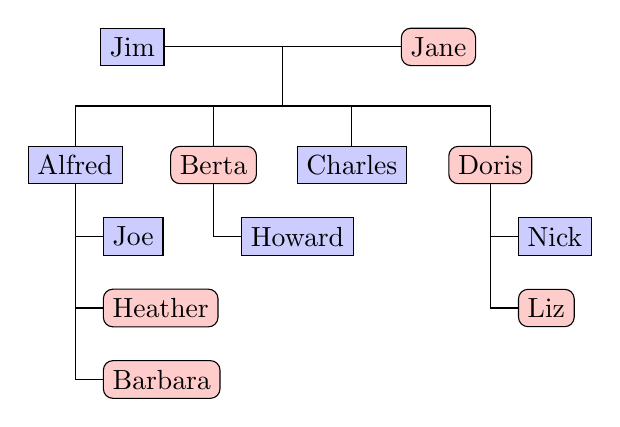
\begin{tikzpicture}[
  man/.style={rectangle,draw,fill=blue!20},
  woman/.style={rectangle,draw,fill=red!20,rounded corners=.8ex},
  grandchild/.style={grow=down,xshift=1em,anchor=west,
    edge from parent path={(\tikzparentnode.south) |- (\tikzchildnode.west)}},
  first/.style={level distance=6ex},
  second/.style={level distance=12ex},
  third/.style={level distance=18ex},
  level 1/.style={sibling distance=5em}]
    % Parents
    \coordinate
      child[grow=left] {node[man,anchor=east]{Jim}}
      child[grow=right] {node[woman,anchor=west]{Jane}}
      child[grow=down,level distance=0ex]
    [edge from parent fork down]
    % Children and grandchildren
    child{node[man] {Alfred}
      child[grandchild,first] {node[man]{Joe}}
      child[grandchild,second] {node[woman]{Heather}}
      child[grandchild,third] {node[woman] {Barbara}}}
    child{node[woman] {Berta}
      child[grandchild,first] {node[man]{Howard}}}
    child {node[man] {Charles}}
    child {node[woman]{Doris}
      child[grandchild,first] {node[man]{Nick}}
      child[grandchild,second] {node[woman]{Liz}}};
\end{tikzpicture}